\newpage
\chapter{Lecture 10/03/2024}

Last lecture we saw that we can approximate a non-linear system with a linear one, locally in an equilibrium point.

Let's consider an electric circuit, if the elecrical field is not static, it generates a variable magnetic field and viceversa. 

$$
\begin{cases}
\Phi = Li \\
Ri = -\dfrac{d\Phi(\vec B)}{dt} = -\dfrac{d(Li)}{dt}
\end{cases}
$$

We can write this system in the cauchy form:

$$
\begin{cases}
\dfrac{di}{dt} = - \dfrac RL i \\
i(0) = i_0
\end{cases}
$$

The solution is:

$$
i(t) = i_0 e^{-\frac Rt}
$$



$$
L \dfrac{di}{dt} + Ri + V_c = 0
$$

$$
VC = Q
$$

$$
y = \begin{bmatrix} i \\ q \end{bmatrix},
\quad
A = \begin{bmatrix}
    -\dfrac{R}{L} & -\dfrac{1}{LC} \\[10pt]
    \phantom{-}1  & \phantom{-}0
\end{bmatrix}
$$

$$
m\ddot x = \gamma \dot x + kx
$$

\newpage

\section{Dirak Delta}

If ypu consider a foorball player that kicks a ball, the force is not constant, and it is not possible to model it with a constant force. We can model it with a Dirak Delta function.

$$
\begin{cases}
m \ddot x = m \dot v = F(t) \\
v(0) = 0
\end{cases}
\quad \Rightarrow \quad
mv_{after} = \int_0^a F(t) dt \quad \Rightarrow \quad \boxed{v_{after} = \dfrac{1}{m} \int_0^a F(t) dt}
$$

So the Dirak Delta function is a function that is zero everywhere except in zero, where it is infinite. It is used to model impulses.

\begin{figure}[H]
    \centering
    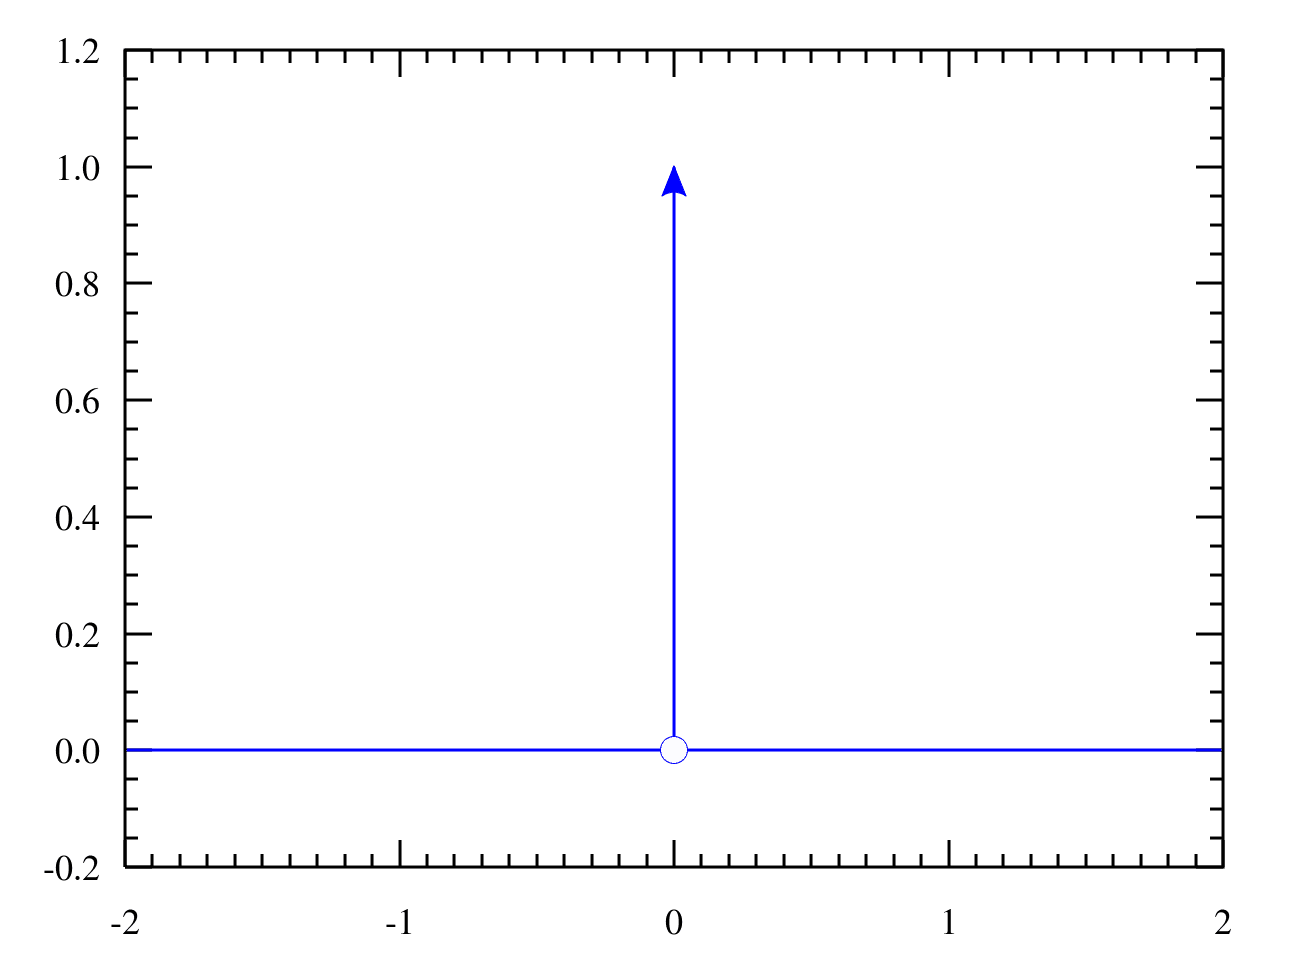
\includegraphics[width=0.5\textwidth]{assets/dirak.png}
    \caption{Dirak Delta Function} \label{fig:dirak}
\end{figure}

\dots

Let's consider a function $f(t)$ such that $f(0) < \infty$ and $f'(0) < \infty$. We can calculate:

$$
\int_{\mathbb R} \delta(t) f(t) dt = \int_{\mathbb R} \delta(t) [f(0) + f'(0)t] dt = \int_{\mathbb R} \delta(t) f(0) dt + \int_{\mathbb R} \delta(t) f'(0)t dt
$$

Now, we use two key properties of the Dirac delta function:
\begin{enumerate}
    \item \textbf{Sifting Property:}
    $$
    \int_{\mathbb{R}} \delta(t) \, dt = 1.
    $$

    \item \textbf{First Moment:}
    $$
    \int_{\mathbb{R}} \delta(t)t \, dt = 0,
    $$

    which follows because \( t\delta(t) \) is an odd function.
\end{enumerate}

Substituting these results, we obtain:

$$
\int_{\mathbb{R}} \delta(t) f(t) \, dt = f(0) \cdot 1 + f'(0) \cdot 0 = f(0).
$$

\dots

\section{Random Processes}

$$
<x(t)> = \dfrac 1N \sum_{i=1}^N {x_R}_i(t)
$$

$$
m_i \ddot x_i = - \gamma \dot x_i
\quad \Rightarrow \quad
m_i \dot v_i = - \gamma v_i 
\quad \Rightarrow \quad
\dot v_i = - \dfrac{\gamma}{m_i} v_i 
\quad \Rightarrow \quad
\boxed{
v_i(t) = v_i(0) e^{-(\gamma / m_i) t}_{\phantom{-\frac 11}}
}
$$

$$
\boxed{
m \dot v = - \gamma v + \hat F_s (t) 
}
$$

$$
m \ddot x = -k\dot x + \hat F_p(x) + \hat F_s(t)
$$
$$
m \ddot x = - k \dot x + k f(x) + k f_s (t)
$$
$$
\dfrac mk \ddot x = - \dot x + f(x) + f_s(t)
$$
$$
\dfrac mk \ddot x \ll 1 \quad \Rightarrow \quad \dfrac mk \ddot x \approx 0
$$
$$
\dot x \simeq f(x) + f_s(t) = f(x) + \omega \xi (t)
$$